% Template Source: This template has been downloaded from:
% http://www.latextemplates.com/template/stylish-article
% License: CC BY-NC-SA 3.0 
%%%%%%%%%%%%%%%%%%%%%%%%%%%%%%%%%%%%%%%%%

%----------------------------------------------------------------------------------------
%	PACKAGES AND OTHER DOCUMENT CONFIGURATIONS
%----------------------------------------------------------------------------------------

\documentclass[fleqn,10pt]{SelfArx} % Document font size and equations flushed left

\usepackage{lipsum} % Required to insert dummy text. To be removed otherwise
\usepackage{svg}
\graphicspath{{images/}}
\usepackage{algorithm}
\usepackage{algpseudocode}
\usepackage{algorithmicx}
\algdef{SE}[DOWHILE]{Do}{doWhile}{\algorithmicdo}[1]{\algorithmicwhile\ #1}
\usepackage{mathtools}

%----------------------------------------------------------------------------------------
%	COLUMNS
%----------------------------------------------------------------------------------------

\setlength{\columnsep}{0.55cm} % Distance between the two columns of text
\setlength{\fboxrule}{0.75pt} % Width of the border around the abstract

%----------------------------------------------------------------------------------------
%	COLORS
%----------------------------------------------------------------------------------------

\definecolor{color1}{RGB}{0,0,90} % Color of the article title and sections
\definecolor{color2}{RGB}{0,20,20} % Color of the boxes behind the abstract and headings

%----------------------------------------------------------------------------------------
%	HYPERLINKS
%----------------------------------------------------------------------------------------

\usepackage{hyperref} % Required for hyperlinks
\hypersetup{hidelinks,colorlinks,breaklinks=true,urlcolor=color2,citecolor=color1,linkcolor=color1,bookmarksopen=false,pdftitle={Title},pdfauthor={Author}}

%----------------------------------------------------------------------------------------
%	ARTICLE INFORMATION
%----------------------------------------------------------------------------------------

\JournalInfo{InnovR 2019} % Journal information
\Archive{4-EII INSA Rennes} % Additional notes (e.g. copyright, DOI, review/research article)

\PaperTitle{Bivariate Function Polynomial Approximation with Dynamic Degree, Real-Time Software Implementation} % Article title

\Authors{Mathieu Percelay\textsuperscript{1}*} % Authors
\affiliation{\textsuperscript{1}\textit{Department of Electronics and Computer Science, INSA Rennes, Rennes, France}} % Author affiliation
 % Author affiliation
\affiliation{*\textbf{Corresponding author}: Mathieu.Percelay@insa-rennes.fr} % Corresponding author

\Keywords{Approximate computing --- Embedded Systems --- Minimum Mean Square Error Method --- Non-uniform Segmentation} % Keywords - if you don't want any simply remove all the text between the curly brackets
\newcommand{\keywordname}{Keywords} % Defines the keywords heading name

%----------------------------------------------------------------------------------------
%	ABSTRACT
%----------------------------------------------------------------------------------------

\Abstract{
The approximation of mathematical functions is an emerging field of research. The needs in embedded systems has never been as much considerable. Many efforts have been made for univariate function approximation. However, regarding multivariate function approximation, only hardware solutions have been proposed. This paper presents a software-oriented polynomial approximation for bivariate functions with a non-uniform segmentation strategy and a dynamic polynomial degree.
}
%----------------------------------------------------------------------------------------

\begin{document}

\flushbottom % Makes all text pages the same height

\maketitle % Print the title and abstract box

\tableofcontents % Print the contents section

\thispagestyle{empty} % Removes page numbering from the first page

%----------------------------------------------------------------------------------------
%	ARTICLE CONTENTS
%----------------------------------------------------------------------------------------

\section{Introduction} % The \section*{} command stops section numbering
Improvements in micro-electronics and the development of the Internet of Things make the amount of Embedded Systems rising sharply. In domains such as telecommunications, signal processing or robotics, mathematical function evaluation is widely used. Even if the computer performances has risen over the past decades, exact
computation is done at the expense of hardware costs, execution time, energy consumption or memory footprint. Such costs can be unsuitable for Real-Time Embedded applications.
It is then possible to reduce the precision of computation, i.e. approximate the function in order to decrease these costs. The challenge is to find the best tradeoff for the application and the hardware target. Approximate-computing is today a very important paradigm \cite{paradigm} in computer science and micro-electronics fields.
Some methods have been previously used as the CORDIC iterative algorithm for trigonometric functions \cite{cordic}, multipartite tables \cite{multipartite} or polynomial approximation \cite{juju}. These methods where developed for univariate function approximation. Some additional issues appear when these methods are extended to multivariate.

To this day, the majorities of multivariate function approximation deals with linear approximation and hardware implementation, by J.Rust et al \cite{encodedgradients} or D. Linaro et al \cite{genetic}. 
The subject of this paper is the study of a software polynomial approximation technique with adaptive methods such as a non-uniform segmentation and a dynamic degree in the idea of being suitable for most applications while maintaining performances. 

The paper is organized as follows. In Section 2 related works on both univariate and multivariate are introduced. Section 3 explains in details the approximation model creation with MATLAB and the C implementation of the evaluation program. Results about the approximation model and the software implementation are discussed in Section 4 before the conclusion in Section 5.
%------------------------------------------------

\section{Related Works}
\subsection{Univariate Polynomial Function Approximation}
The starting point of the works presented in this paper is the method proposed by J. Bonnot in \cite{juju}. The paper presents a smart univariate polynomial approximation method. It is combined with a non-uniform segmentation method and a fixed point coefficient encoding.
The approximating polynomial is found through the Remez algorithm which minimizes the maximum error between the polynomial and the approximated function.
An error criterion has to be observed and if it is not, a segmentation of the function domain is performed. A new polynomial is computed on each of the two resulting sub-segments. If the criterion is still unsatisfied, the process is repeated recursively.

The degree is fixed for all polynomials and given at the begin of the process.

That segmentation is then represented in a binary tree which is then reduced by a memory saving strategy.
This way of segmentation allows an efficient most-significant-bit indexing when evaluating the approximating polynomial and a very concise representation.

\subsection{Hardware-Oriented Bivariate Linear Approximation}
In \cite{encodedgradients} are presented interesting methods about the segmentation with two variables function. The function is linearly approximated, i.e. approximated by a bivariate polynomial of degree 1. The coefficients of this polynomial are computed through the Minimum Mean Square Error (MMSE) Method.
A bivariate non-uniform segmentation similar to the univariate case in \cite{juju} is performed. If the error criterion is not observed, the original segment is split into four equal squared subsegments. 

When the recursive process is terminated, a segment merging step is considered. A merging between two segments is performed when they are neighbors, i.e. they have a complete side in common, and the approximation created by the mean of their coefficients observes the error criterion on the whole segment.
An example of such a segmentation is shown in Figure \ref{merging}.

\begin{figure}[h]
    \centering
    \includegraphics[width=\columnwidth]{graphics/merging.png}
    \caption{An example of a non uniform segmentation with merging. (I, IV) and (VI, VII) have been merged}
    \label{merging}
\end{figure}

\section{Proposed Solution}
In order to overcome the lack of software-oriented solutions of polynomial bivariate-function approximation, 
the proposed method aims to offer an efficient and adaptive technique for the higher number of applications. This technique is based on 
the Mean Square Minimization Method which is appropriate for the majority of approximation problems.
This solution uses a smart non-uniform segmentation in order to better fit irregularities of the approximated function.
Furthermore, for best performances, the degree of the bivariate approximating polynomial is dynamic which avoid data and time waste.
The proposed method is split into two step. The first step is the Approximation Model Creation which compute the polynomial coefficients and space segmentation for the desired approximated function with MATLAB. The second step is the use of this approximation model in a Real-Time-oriented embedded system with an optimized C-software.

\subsection{Approximation Model Creation with MATLAB}
\subsubsection{Mean Square Minimization Method Adaptation}%TODO définir un point
Let consider a bivariate function $f$ defined on a space $E$.
$$\begin{array}{cccccc}
	f & : & E \subset \mathbb{R}^2 & \to & \mathbb{R}\\
      &   & p = (x, y) & \mapsto & f(p) \\
	\end{array}$$
The Mean Square Minimization method will be used as follow. An uniformly segmented rectangular space is considered which will be given by $n$ points $\{p_i = (x_i, y_i) \in E , i = 1..n \}$.
Let be $m$ bivariate monomials
$$\left \{
\begin{array}{cccccc}
M_i & : & E          & \to     & \mathbb{R} & i = 1..m \\
    &   & p = (x, y) & \mapsto & x^{a_i}\times y^{b_i} & a_i, b_i \in \mathbb{N} \\
\end{array}
 \right \}$$
and $m$ coefficients $\{\alpha_i \in \mathbb{R}, i = 1..m \}$. The corresponding bivariate polynomial $P$ is defined as follow :
$$\begin{array}{cccccc}
	P & : & E  & \to & \mathbb{R}\\
      &   & p = (x, y) & \mapsto & \sum_{i=1}^{m}{\alpha_i \times M_i(p)} \\
	\end{array}$$
The goal is to find the right $\alpha_i s$ in order to get a statisfying approximation if $f$ by $P$. Such a solution can be find by the \emph{Minimum Mean Square Error Method} (MMSE). 
Let be 

$$A\in \mathbb{R}^{n\times m} = 
\begin{pmatrix}
   M_1(p_1) & \cdots & M_m(p_1)\\
   \vdots   & \ddots & \vdots  \\
   M_1(p_n) & \cdots & M_m(p_n) 
\end{pmatrix}$$

$\alpha \in \mathbb{R}^m = 
\begin{pmatrix}
   \alpha_i \\
   \vdots \\
   \alpha_m
\end{pmatrix}$
 and
$F \in \mathbb{R}^n = 
\begin{pmatrix}
   f(p_1) \\
   \vdots \\
   f(p_n)
\end{pmatrix}$

The Mean Square Error (MSE) of the approximation of $f$ by $P$  problem is : $MSE = \|(A\alpha - F)^2\|$. The \emph{MMSE} Method gives the solution $\tilde{\alpha}$ of the \emph{MSE} minimum by solving the equation $A^T A \tilde{\alpha} = A^T F$.

The degree of a polynomial is defined as : $d = max(a_i + b_i), 1_i)$ \cite{polynomials}. For a a given degree $d$, there is $m = \frac{(d+1)d}{2}$ different monomials of degree $\leq d$. The corresponding polynomial $P$ is of degree $d$. The proposed technique uses polynomials characterized by their degree, which can be dynamic, in other words, different for each polynomial used.
The monomials $M_i$ have to be memorized in a known order as described in Figure \ref{tree_mapping}, in order to rebuild the polynomial $P$ well.

\begin{figure}
    \centering
    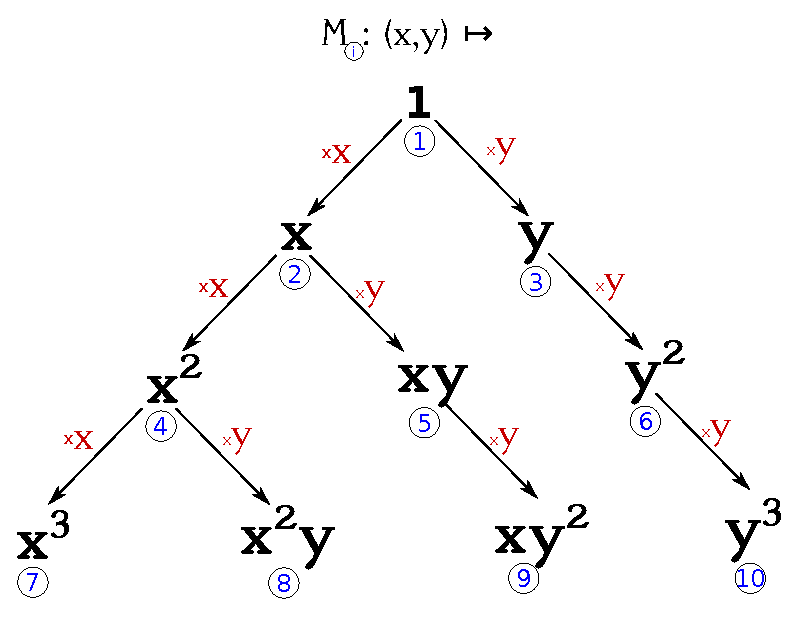
\includegraphics[width=\columnwidth]{graphics/tree_mapping.eps}
    \caption{The way of computation of the monomials for a polynomial of degree 3. Each \emph{i}th monomial is deduced from the previous one according to the nodes ordering in the tree.}
    \label{tree_mapping}
\end{figure}

The MSE is then compared with a criterion $\epsilon$. If it is not respected (ie. $MSE \geq \epsilon$), a segmentation is done.

\subsubsection{Sufficient Degree Segmentation Method}
To match irregularities of $f$, a segmentation of $E$ can be useful. Segmenting $E$ means splitting it in several subsets $Es_i$ and the same MMSE Method is applied on these subsets to solve the minimization problem. The solution to the global problem on $E$ is equal to the union of the solution on each $Es_i$.
For the proposed technique, the segmentation is implemented as a four regular quadrant splitting for performances and implementation ease. For $E = [a, b]\times [c, d]$ : 
\begin{equation}
 Es = \begin{dcases*}
        Es_1 = [a, \frac{a+b}{2}] \times [c, \frac{c+d}{2}]\\
		Es_2 = [\frac{a+b}{2}, b] \times [c, \frac{c+d}{2}]\\
		Es_3 = [a, \frac{a+b}{2}] \times [\frac{c+d}{2}, d]\\
		Es_4 = [\frac{a+b}{2}, b] \times [\frac{c+d}{2}, d]
        \end{dcases*}
        \label{subE}
\end{equation}

The segmentation can be applied recursively on one or several subsets. The segmentation scheme becomes then a non-uniform segmentation which is described with a quadtree as shown in Figure \ref{seg_tree}.
Each node of the tree is containing the coefficients vector $\alpha$ computed by the MMSE Method on a given segment. The degree of $P$ can be different, so the length of $\alpha$ is dynamic according to the considered segment.


The Sufficient Degree Segmentation Method as for input 
\begin{itemize}
    \item a function $f$ and its domain of definition $E$
    \item a MSE criterion $\epsilon$
    \item a degree limit $d_{max}$
\end{itemize}

Then the method uses the MMSE Method as described in the previous section according to the recursive algorithm Alg.\ref{alg:suff}
\begin{algorithm}
\begin{algorithmic}[1]
\Function{$SDS$}{$f, E, \epsilon$}
\State $d \gets 0$
\Do
	\State $\alpha \gets polynomial\_least\_square(f, E, d)$ 
	\State $MSE \gets get\_MSE(f, E, \alpha)$
    \State $d \gets d+1$
\doWhile{$MSE > \epsilon $ and $d \leq d_{max}$}
\State $t \gets tree(\alpha)$
\If{$MSE > \epsilon$}
	\For{$e \in segmentation(E)$}
		\State $t \gets add\_subtree(t, SDS(f, e, \epsilon))$
	\EndFor
\EndIf \\
\Return $t$
\EndFunction
\end{algorithmic}
\caption{Sufficient Degree Segmentation (SDS) Algorithm}
\label{alg:suff}
\end{algorithm}

The final approximating polynomial model is given by the segmentation tree and the corresponding polynomial coefficients given by the MMSE Method for each segment.
\begin{figure*}
\centering
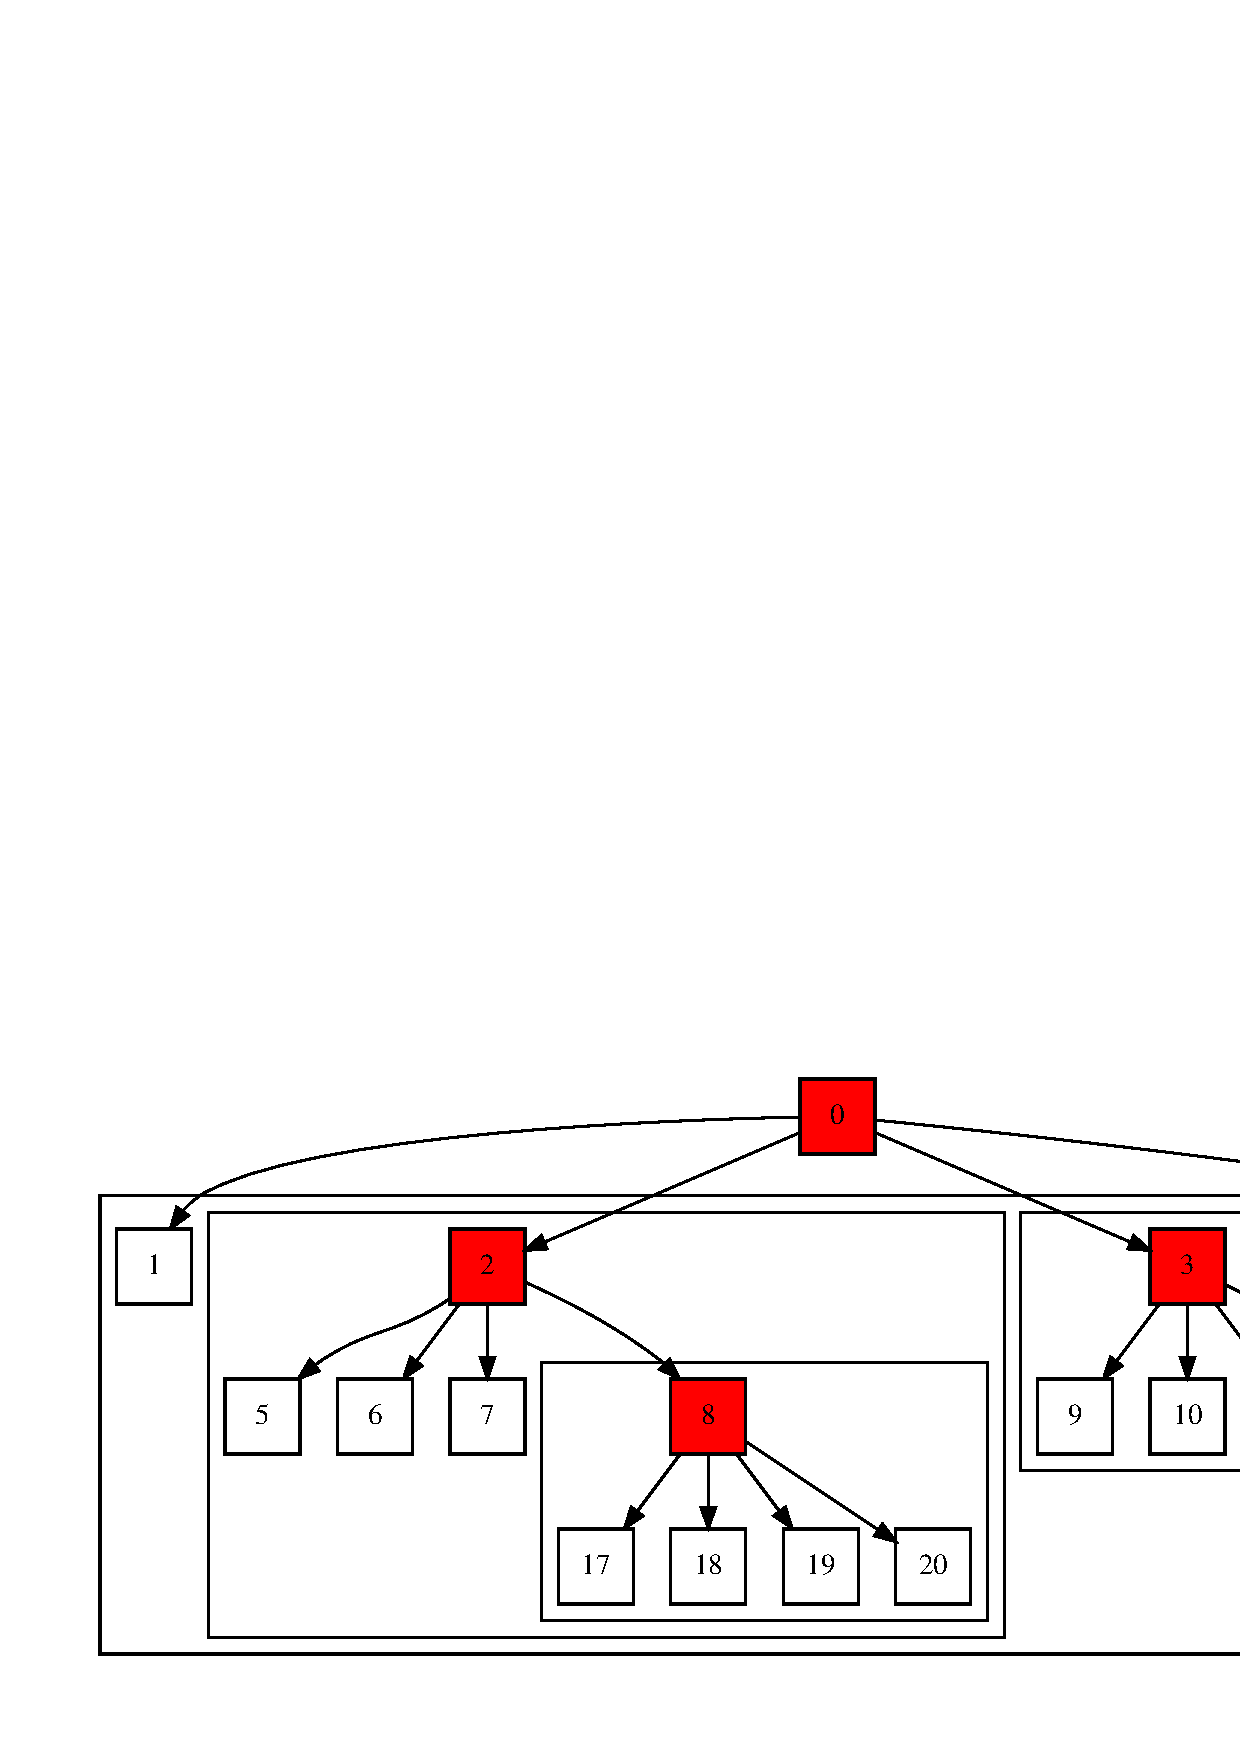
\includegraphics[width=\columnwidth]{graphics/seg_tree.pdf}
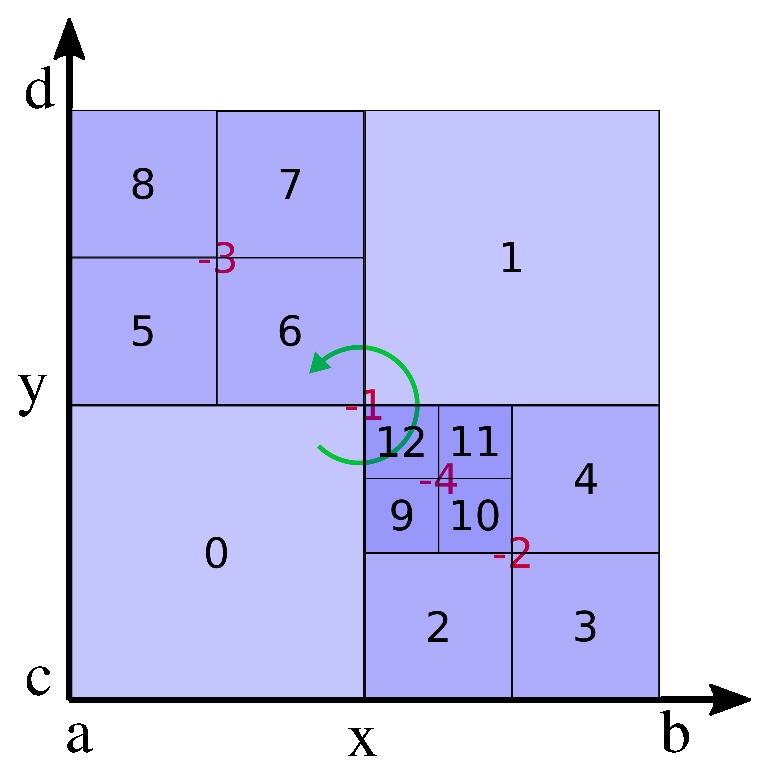
\includegraphics[width=0.7\columnwidth]{graphics/segmentation.eps}
\caption{Example of segmentation tree}
\label{seg_tree}
\end{figure*}

\subsubsection{Best Tradeoff Segmentation Method}
The previous method is a naive sufficient solution search. This solution might not be satisfying because the memory footprint is too big or the evaluation latency is too long. These two important data in embedded systems are considered in the Best Tradeoff Segmentation Method. 

The memory footprint is computed from the data needed for the segmentation tree representation and from the polynomial coefficients storage.
The latency is estimated in number of elementary operations. It takes in account the segmentation tree traversing and the evaluation using the polynomial coefficients. As each algorithmic operation (addition, multiplication, comparison, memory access) have different latencies according to the hardware target so these parameters have to be estimated previously.
Given the limits $m_{max}$, $t_{max}$ and $\epsilon$ which are respectively the maximum footprint, the maximum latency and the maximum MSE desired.

The Best Tradeoff Method looks for a satisfying solution respecting these limits through an exhaustive research in all the configurations of the segmentation tree and the polynomial degrees. This exhaustive research is done until a maximum tree depth $s_{max}$ and a maximum polynomial degree $d_{max}$ for performances and in case of no satisfying solution.

\subsection{Real-Time-oriented Software Evaluation}

Once the adapted approximation model has been found through the previously detailed methods, it needs to be translated in a Embedded-Oriented software language. For best performances, the C language has been chosen.

\subsubsection{Efficient Model Description in C with floating point}
The first item to depict is the segmentation tree.
A Breadth First Search (BFS) is performed in the segmentation tree in order to number the nodes. The numbering is different according to the node nature : leaf or father. A father is a node where the MMSE solution $\alpha$ is not satisfying and the segment has been divided. A leaf is a final node where $\alpha$ describes a polynomial function $P$ that respects the MSE criterion $\epsilon$ with $f$ for the sub-segment.
For each depth, the four neighboring nodes are counterclockwise numbered starting with the first one as described in equation \ref{subE}.
One table $T_{leaf}$ is created with this numbering and is indexed by the order given by the BFS.
Given $x$ and $y$ the function arguments expressed in floating point representation, the leaf corresponding to the segment which includes $x$ and $y$ can be found with Algorithm \ref{alg:tree_traversal} with $index = 0$, the root of the tree.
\begin{algorithm}
\begin{algorithmic}[1]
\Function{$leaf = FindLeaf$}{$T_{leaf}, index, x, y$}
\If{$T_{leaf}[index] < 0$}
	\State $firstQuadrant \gets (T_{leaf}[index] -1)*4+1$
	\State $q = FindQuadrant(T_{leaf}, index, x, y)$
	\State \Return $FindLeaf(T_{leaf}, firstQuadrant+q, x, y)$
\Else
	\State \Return $T_{leaf}[index]$
\EndIf
\EndFunction
\end{algorithmic}
\caption{Segmentation Tree Traversal Algorithm}
\label{alg:tree_traversal}
\end{algorithm}

$leaf$ indexes two other tables $T_{first\_\alpha}$ and $T_d$ which indicate respectively the index of the first coefficient of the segment in the table $T_{\alpha}$ and the degree of the approximating polynomial $P$. $T_{\alpha}$ contains the concatenation of all the coefficients in floating point representation. $\alpha$ is then reconstructed.
\begin{equation*}
\begin{cases}
first\_\alpha = T_{first\_\alpha}[leaf]\\
d = T_d[leaf] \\
\alpha = T_{\alpha}[first\_\alpha:first\_\alpha+NB\_\alpha(d)]
\end{cases}
\end{equation*}

The monomials $M$ are computed as it was done in Figure \ref{subE} according to the degree $d$. The monomials are then multiplied by there respective coefficient in $\alpha$ and added up.
\begin{equation*}
P(x, y) = \sum_{i = 1}^{NB\_\alpha(d)} \alpha_i \times M_i \approx f(x, y)
\end{equation*}

%------------------------------------------------
\section{Results and Discussion}
\subsection{peaks MATLAB example function}
The \emph{peaks} MATLAB bivariate example function is very useful for segmentation visualization with their irregularities. It is also a function hard to evaluate with classical mathematical function toolboxes as \emph{libm} due to the presence of exponential and square functions.
\begin{equation*}
\begin{split}
peaks(x, y) = & 3\times (1-x)^2 \times e^{-x^2 - (y+1)^2} - 10 \times (\frac{x}{5} - x^3 - y^5) \\
              & \times e^{-x^2-y^2} - \frac{1}{3} \times e^{-(x+1)^2 - y^2}
\end{split}
\end{equation*}

A visual example of the approximation model and the original function is presented in Figure \ref{peaks}. 
\begin{figure*}[h]
\centering
\includegraphics[width=0.8\linewidth]{graphics/peaks.eps}
\caption{peaks approximation function for $\epsilon = 0.001$, $d_{max} = 4$ and $s_{max} = 6$}
\label{peaks}
\end{figure*}

A series of tests has been performed on a ARM Cortex A53 processor with the C implementation presented and the Best Tradeoff Method. The Figure \ref{results} shows them.
When $d_{max}$ if small, in order to to respect the error criterion, the segmentation is very fine and needs a lot of memory to be represented. The evaluation time is on the contrary small because there is few coefficient then few floating point operations to process. 
When $d_{max}$ is increasing, the memory footprint is decreasing but the evaluation is longer.
Once $d_{max} \geq 5$, the model does not change because the Best Tradeoff Method found that the minimum of memory footprint is reached.

\begin{figure}[h]
\centering
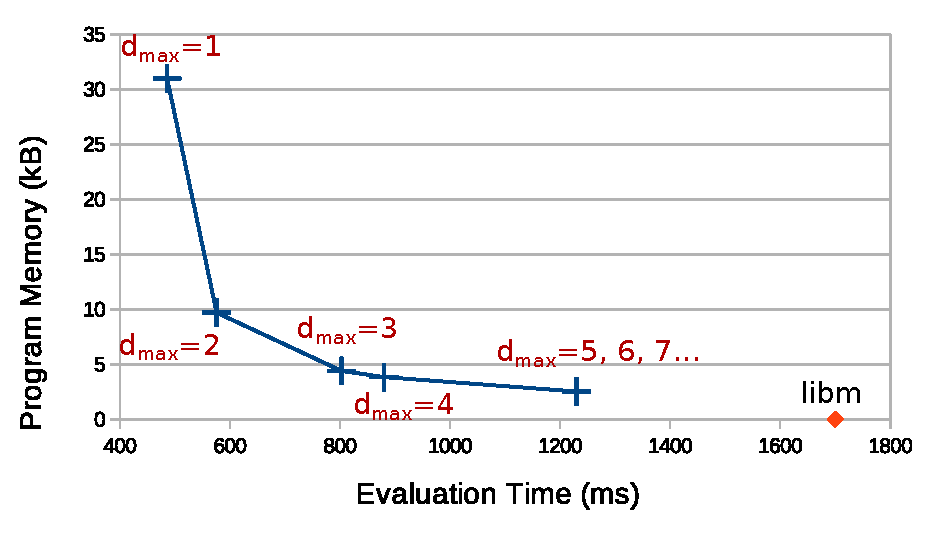
\includegraphics[width=\columnwidth]{graphics/results.eps}
\caption{Results for evaluation of 1 million points uniformly distributed with $f=peaks$, $E = [-3,3]\times[-3,3]$, $\epsilon = 0.001$ and $s_{max} = 6$}
\label{results}
\end{figure}


\section{Conclusion}
In this paper, an adaptative technique for efficient bivariate function polynomial approximation has been presented thanks to a non-uniform segmentation strategy and a dynamic degree solution. A software implementation shows the efficiency of the proposed technique with a bivariate function example on an ARM Cortex A53 processor, designed for very low consumption applications.
This implementation uses floating point arithmetic for both segmentation tree traversal and coefficient encoding. The floating point processing is often inefficient in embedded systems due to calculation costs. A fixed point solution must be considered for future work.

%------------------------------------------------
\section*{Acknowledgments} % The \section*{} command stops section numbering
The author wishes to thank J. Bonnot and D. Ménard for their previous works and their helpful comments and discussions. 

%----------------------------------------------------------------------------------------
%	REFERENCE LIST
%----------------------------------------------------------------------------------------
\phantomsection
\bibliographystyle{unsrt}
\bibliography{sample}

%----------------------------------------------------------------------------------------

\end{document}
